\documentclass[11pt,letterpaper]{article}
\usepackage[margin=.78in]{geometry}
\usepackage[T1]{fontenc}
\usepackage{lmodern,booktabs,graphicx,amsmath,amssymb,xcolor,microtype,hyperref,titlesec}
\usepackage{fancyhdr}
\definecolor{ink}{HTML}{19353A}
\definecolor{muted}{HTML}{456166}
\hypersetup{colorlinks=true,urlcolor=ink,linkcolor=ink,citecolor=ink,pdfauthor={Robert Jahnke},pdftitle={Regional inference for a frozen Fast Feature Field}}
\setlength{\parindent}{0pt}
\setlength{\parskip}{5pt}
\setlength{\headheight}{14pt}
\pagestyle{fancy}
\fancyhf{}
\fancyhead[L]{\small\color{muted}REGIONAL INFERENCE FOR F3}
\fancyhead[R]{\small\color{muted}24 November 2026}
\fancyfoot[R]{\small\color{muted}\thepage}
\titleformat{\section}{\large\bfseries\color{ink}}{\thesection}{.55em}{}
\titleformat{\subsection}{\normalsize\bfseries\color{ink}}{\thesubsection}{.55em}{}
\titlespacing*{\section}{0pt}{9pt}{3pt}
\titlespacing*{\subsection}{0pt}{6pt}{2pt}
\renewcommand{\arraystretch}{1.12}
\newcommand{\repo}{https://github.com/RobertAris/f3-regional-inference}
\begin{document}
{\LARGE\bfseries\color{ink}Regional inference for a frozen Fast Feature Field\par}
{\large Robert Jahnke}\par
\textbf{Abstract.}
Fast Feature Field (F3) builds a dense representation from camera events. We ask how much work can be avoided when the caller already knows which pixels it needs. We keep an exact encoder prefix, estimate the remaining image-wide normalization factors on a coarser grid, and evaluate the requested regions at native resolution. On one Apple M5 Max, ten feature-and-flow regions arrived 7.72--8.84\% sooner on average across four panels than the fastest measured dense method with finite output. Four of 430 regions exceeded 0.50 px flow disagreement with dense F3. Feature-only requests also saved time on two of three sensors, with some loss of fidelity. Exact regional decoding had little effect on depth latency, and an equally optimized dense segmentation decoder was faster on all 18 packets tested at FP16.

\section{Computing global normalization for a local query}
The \href{https://arxiv.org/html/2509.25146v2}{Fast Feature Field of Das, Daniilidis and Chaudhari} maps events to a 32-channel feature field shared by downstream heads. Its encoder has six convolutional blocks. The flow head adds four more. Each uses global response normalization (GRN). For pre-normalization activation $u_\ell(p,c)$ in channel $c$, the factor is
\[
 g_\ell(c)=\frac{\|u_\ell(\cdot,c)\|_2}
                  {C_\ell^{-1}\sum_j\|u_\ell(\cdot,j)\|_2+10^{-6}}.
\]
An input crop changes the sum even if every convolutional neighbor of a query is present. Once the ten factor vectors are known, a 34-pixel halo supplies all the required convolutions. Computing those vectors exactly incurs full-frame work.

For flow we run five encoder blocks over the native packet. A stride-two preview samples the sixth block's first convolution on that native map. For later convolutions, if $U$ interpolates a coarse input onto the native grid, the preview filter is $U^\top w$. This preserves the linear response $\langle w,Ux\rangle$ on interpolated inputs. Sampling and nonlinearities still introduce error. With the five estimated factors, the original kernels finish the requested features and flow using a 19-pixel halo and native image padding. The timing comparison uses FP32 and bicubic projection.

\subsection{Which approximation matters?}
An earlier FP32 bilinear experiment held the five-block native prefix, stride and requested regions fixed. The entries below are flow-component RMS differences from dense FP32, in pixels.

\begin{center}\small
\begin{tabular}{@{}lrr@{}}\toprule
Preview & M3ED & Prophesee EVIMO2v2\\\midrule
Ordinary coarse filters & 0.684 & 1.208\\
Native first response only & 0.744 & 1.040\\
Scale-corrected filters only & 0.094 & 0.326\\
Native first response and scale-corrected filters & 0.053 & 0.089\\\bottomrule
\end{tabular}\end{center}
Filter scale explains most of the improvement. Sampling the first response on the native map helped both panels once the later filters had the correct scale. Transferring thumbnail statistics to native patches and transforming filters across scales have precedents in \href{https://arxiv.org/abs/2103.11784}{Thumbnail Instance Normalization} and \href{https://arxiv.org/pdf/1411.6369}{SiCNN, Eq.~8}. Here these operations estimate the specific GRN factors that couple distant F3 outputs.

\newpage
\section{Fresh feature-and-flow requests}
Each request returned ten $32\times32$ rectangles from one 20 ms packet, including all 32 features and both flow components as FP32 arrays on the host. Six rectangle slots per resolution had fixed coordinates and four followed sampled events. Each of 43 previously studied recordings supplied its earliest archived test window. The regional configuration and original comparison rules were fixed using other windows from the same recordings. This measures transfer across windows in known recordings.

Weights were resident on an M5 Max. Timing included event accumulation, the network and synchronized host delivery. Region selection, rectification, loading and disk I/O preceded the timer. No results from the current packet were cached. Five warmed, interleaved repetitions gave a median for each method and packet. Dense candidates combined FP16 or FP32 with a matched implementation, the released full-host path, or the released path with a device-side gather.

\begin{center}\small
\begin{tabular}{@{}lrrrl@{}}\toprule
& & \multicolumn{2}{c}{Mean latency saved} & 95\% interval\\
\cmidrule(lr){3-4}
Panel & Recordings & All finite & Within tolerance & Within tolerance\\\midrule
Prophesee EVIMO2v2 & 14 & 8.35\% & 13.17\% & [9.48, 16.85]\%\\
Samsung EVIMO2v2 & 16 & 8.70\% & 10.29\% & [8.54, 13.60]\%\\
M3ED & 6 & 8.84\% & 8.84\% & [7.10, 10.40]\%\\
E-MOTION & 7 & 7.72\% & 7.72\% & [6.51, 8.78]\%\\\bottomrule
\end{tabular}\end{center}
The original comparator selected the fastest dense candidate on each packet with feature relative RMS at most 1.5\% and flow-component RMS at most 0.50 px against dense FP32. A retrospective sensitivity analysis admitted any dense candidate with finite output. The original screen excluded a faster dense candidate on five Prophesee and two Samsung packets. Regional inference still finished sooner on all 43 packets.

Savings average the paired ratios $1-t_{\rm regional}/t_{\rm dense}$. Captures receive equal weight within a physical setup and setups receive equal weight within a panel. The EVIMO2v2 panels have five Prophesee and four Samsung setups. M3ED and E-MOTION use recordings as units. The original intervals use 20,000 paired bootstrap resamples of these units. They quantify variation within the measured workload.

\subsection{Four errors at the image boundary}
The original study required every packet to satisfy both tolerances. Only 42/43 did when averaged over ten regions. Evaluated separately, every region passed on 40/43 packets. All 430 met the feature limit, with a maximum relative RMS difference of 0.215\%. Four corner regions exceeded the flow limit. Two Samsung upper-left corners reached 2.09 and 1.01 px. Two corners on one E-MOTION packet reached 0.98 and 0.76 px.

On those three packets we replaced the estimated factors with the exact full-frame factors and reran the same regional suffix. All ten regions on each packet agreed with the matched dense path. The largest flow RMS difference from the released dense path fell below $5\times10^{-6}$ px. This retrospective substitution isolates the normalization approximation in those failures. It requires a dense pass. The four panels establish a latency saving on this device and leave a measurable risk of local error.

\vfill\small\href{\repo/blob/main/docs/reproduction.md}{Timing records and protocols}
\enspace$\cdot$\enspace\href{\repo/blob/main/evidence/benchmarks.zip}{Per-region errors and substitution experiment}\normalsize
\newpage
\section{Requests for features alone}
For four $48\times48$ regions chosen from current event activity, we varied the number of exact native encoder blocks. The output was the same set of 32-channel native feature tiles for all implementations. The primary feature-only configuration kept three blocks at native resolution. This left a nine-pixel halo around each requested core. A batch can share the surrounding computation when regions overlap.

Development used separate recordings to select the split and stride. Each evaluation recording contributed three predetermined packets, with three interleaved timing repeats per method. Timing included selecting regions and delivering the results to the host. The same recordings contribute multiple packets. The mean field error below is the RMS difference relative to the FP32 dense signal on the requested pixels.

\begin{center}\small
\begin{tabular}{@{}lrrrrr@{}}\toprule
& & \multicolumn{2}{c}{Latency (ms)} & \multicolumn{2}{c}{Field error (\%)}\\
\cmidrule(lr){3-4}\cmidrule(l){5-6}
Panel & Packets & Regional & Dense FP16 & Regional & Dense FP16\\\midrule
MVSEC & 15 & 10.88 & 10.25 & 1.31 & 1.11\\
DSEC & 24 & 47.73 & 49.77 & 1.00 & 0.56\\
M3ED & 18 & 137.63 & 150.19 & 1.05 & 0.65\\\bottomrule
\end{tabular}\end{center}
Regional inference saved 4.11\% on DSEC and 8.36\% on M3ED. It was faster on every measured packet in those two panels, but only eight DSEC and four M3ED packets also had field error as low as dense FP16. MVSEC favored dense FP16 on all 15. An uncorrected stride-two preview on DSEC took 44.97 ms with 2.63\% field error. Sampling the first response on the native grid and projecting the later filters brought latency to 47.73 ms and error to 1.00\%.

\begin{center}
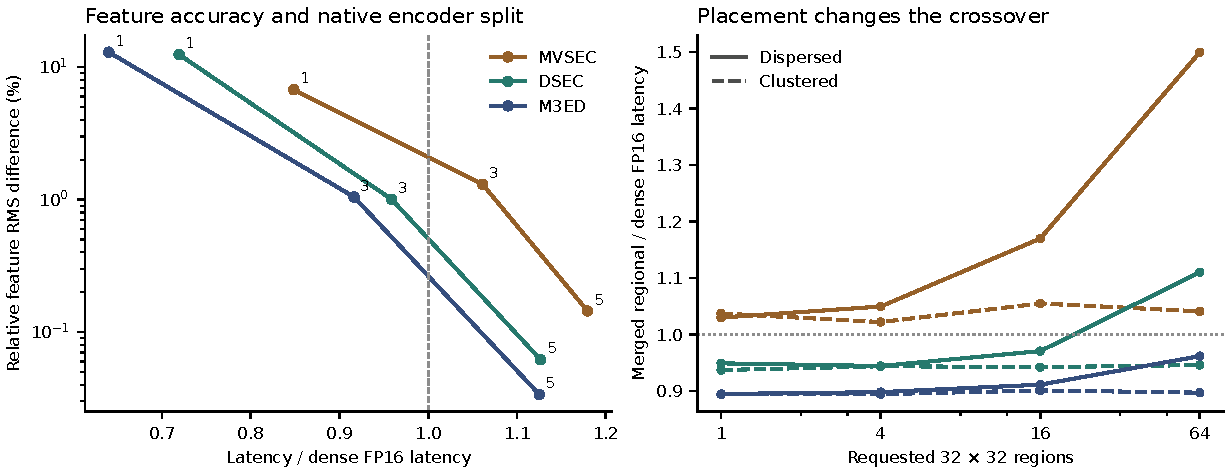
\includegraphics[width=.97\linewidth]{figures/feature-crossover.pdf}
\end{center}
{\small\color{muted}Left, four event-selected regions. Numbers indicate the count of native prefix blocks. Right, one packet per sensor with clustered or dispersed requests. A ratio below one favors the regional path.}

On the sampled DSEC packet, the regional path crossed dense FP16 between 16 and 64 dispersed $32\times32$ requests. It remained faster at 64 clustered requests, which share output pixels and halos. The sampled sensors gave different crossovers. Dense FP16 is a strong alternative when its numerical error is acceptable. Sensor resolution, event count and scene content vary together across the three evaluation panels.

\newpage
\section{Downstream heads and ground truth}
Relative depth uses DINOv2 with global attention and a DPT decoder. Exact regional inference keeps the global field and transformer, then evaluates the final convolution and interpolations on the requested support. SegFormer B3 also retains its global stages. We combine each pointwise stage projection with its fusion weights before interpolation and apply the classifier after summation. This order of multiscale fusion has a direct precedent in \href{https://openaccess.thecvf.com/content/CVPR2023/papers/Hu_You_Only_Segment_Once_Towards_Real-Time_Panoptic_Segmentation_CVPR_2023_paper.pdf}{Hu et al., CVPR 2023, \S3.2}. The same simplification applies to the dense comparator.

At matched FP32 the regional depth path took 97.08 versus 95.44 ms on MVSEC and 284.07 versus 284.86 ms on M3ED. All 33 packets agreed with dense within $1.3\times10^{-6}$ relative RMS. The fully FP16 configuration gave nonfinite outputs on all 33. The dense FP16 encoder with an FP32 head remained finite and faster. A matching mixed-precision regional run is missing. FP32 semantic labels agreed at every requested pixel on 18 packets. At matched FP16 the optimized dense decoder won all 18 timing comparisons, by 3.44 ms on manual night labels and 3.13 ms on daytime pseudo-labels on average.

\subsection{How much can image position predict?}
We retrospectively scored image-row predictions on the same union of valid, requested pixels. For depth, increasing image row predicts increasing inverse depth with no fitting. For semantics, each row predicts its most common class in the three masks of that domain's development take. We average depth rank correlations over packets and compute semantic mIoU from pooled confusion counts.

\begin{center}\small\begin{tabular}{@{}lrrrl@{}}\toprule
Panel & Valid pixels & Image row & Dense F3 & Metric\\\midrule
MVSEC, 15 packets & 97,478 & 0.682 & 0.496 & Spearman $\rho$\\
M3ED, 18 packets & 4,559 & 0.330 & 0.576 & Spearman $\rho$\\
DSEC manual night, 9 packets & 72,431 & 10.52 & 23.91 & mIoU (\%)\\
DSEC pseudo-labels, 9 packets & 81,853 & 8.34 & 33.07 & mIoU (\%)\\\bottomrule
\end{tabular}\end{center}
Even ordinary coarse depth on MVSEC ($\rho=0.608$) ranked below the image-row cue. M3ED favored F3, with as few as 11 valid depth pixels in one packet. The semantic model improved over the row prior in both domains. The manual masks come from three takes on one night route. Native sensor resolution differs from the upstream semantic validation canvas. Stereo and depth used packets centered on the label time, including 10 ms of later events.

\subsection{When a simpler method is enough}
Event-count SGBM on DSEC gave 6.18 px disparity MAE in 20.90 ms versus 7.68 px in 98.54 ms for our sparse F3 matcher, using zero disparity for missing returns on common support. The original F3 paper also used PCA features with SGBM. These timings concern our patch matcher. On high-resolution future occupancy, past event frequency scored 0.091 bits per bin versus 0.835 for regional F3's uncalibrated output. An earlier moving-object reader preserved F3 mask IoU within 0.02 percentage points and saved 17.51 ms, but a raw-event reader attained higher IoU.

F3 already shares its field across tasks. For five outputs on one DSEC packet, shared dense took 194.54 ms and shared regional took 200.11 ms (5.15 and 4.99 serial packets/s, respectively). Peak sampled Metal driver allocations were 2,228 and 2,232 MiB. Recomputing the encoder for separate services took 428.28 ms. The evidence for selective execution is strongest for a few feature or feature-and-flow requests whose consumer needs the learned field. Hardware transfer and an improvement in a closed-loop application remain open.

\vfill\small\href{\repo/blob/main/docs/reproduction.md}{Reproduction guide}
\enspace$\cdot$\enspace\href{\repo/blob/main/evidence/tables.md}{Full benchmark tables}
\enspace$\cdot$\enspace\href{\repo/blob/main/evidence/spatial-controls.json}{Image-row controls}
\end{document}
